\documentclass[conference]{IEEEtran}
\IEEEoverridecommandlockouts
% The preceding line is only needed to identify funding in the first footnote. If that is unneeded, please comment it out.
\usepackage{cite}
%\usepackage[square,sort,comma,numbers]{natbib}
\usepackage{amsmath,amssymb,amsfonts}
\usepackage{algorithmic}
\usepackage{graphicx}
\usepackage{subfigure}
\usepackage{colortbl}
\usepackage{textcomp}
\usepackage{xcolor}
\def\BibTeX{{\rm B\kern-.05em{\sc i\kern-.025em b}\kern-.08em
    T\kern-.1667em\lower.7ex\hbox{E}\kern-.125emX}}
\begin{document}

\title{Identifying functional evolution processes according to the pathological stages of colorectal cancer}
%Identification of pathways related to the four stages of colorectal cancer}
%\author{\IEEEauthorblockN{1\textsuperscript{st} Given Name Surname}
%\IEEEauthorblockA{\textit{dept. name of organization (of Aff.)} \\
%\textit{name of organization (of Aff.)}\\
%City, Country \\
%email address}
%\and
%\IEEEauthorblockN{2\textsuperscript{nd} Given Name Surname}
%\IEEEauthorblockA{\textit{dept. name of organization (of Aff.)} \\
%\textit{name of organization (of Aff.)}\\
%City, Country \\
%email address}
%\and
%\IEEEauthorblockN{3\textsuperscript{rd} Given Name Surname}
%\IEEEauthorblockA{\textit{dept. name of organization (of Aff.)} \\
%\textit{name of organization (of Aff.)}\\
%City, Country \\
%email address}
%\and
%\IEEEauthorblockN{4\textsuperscript{th} Given Name Surname}
%\IEEEauthorblockA{\textit{dept. name of organization (of Aff.)} \\
%\textit{name of organization (of Aff.)}\\
%City, Country \\
%email address}
%\and
%\IEEEauthorblockN{5\textsuperscript{th} Given Name Surname}
%\IEEEauthorblockA{\textit{dept. name of organization (of Aff.)} \\
%\textit{name of organization (of Aff.)}\\
%City, Country \\
%email address}
%\and
%\IEEEauthorblockN{6\textsuperscript{th} Given Name Surname}
%\IEEEauthorblockA{\textit{dept. name of organization (of Aff.)} \\
%\textit{name of organization (of Aff.)}\\
%City, Country \\
%email address}}

\author{
\IEEEauthorblockN
{
	Bolin Chen\IEEEauthorrefmark{2}\IEEEauthorrefmark{4},
	Manting Yang\IEEEauthorrefmark{2}, 
	Li Gao\IEEEauthorrefmark{2} and
	Xuequn Shang\IEEEauthorrefmark{2}\IEEEauthorrefmark{4}\IEEEauthorrefmark{1}
}\\
%
\IEEEauthorblockA{\IEEEauthorrefmark{2} School of Computer Science, Northwestern Polytechnical University, Xi'an, China}
%
\IEEEauthorblockA{\IEEEauthorrefmark{4}Key Laboratory of Big Data Storage and Management, Ministry of Industry and Information Technology, \\
Northwestern Polytechnical University, Xi'an, China}
%
%\IEEEauthorblockA{\IEEEauthorrefmark{5}Key Laboratory of Big Data Storage and Management, Ministry of Industry and Information Technology, \\
%Northwestern Polytechnical University, Xi'an, China}
 \IEEEauthorrefmark{1}Corresponding email: npu\_bioinf@hotmail.com}



\maketitle

\begin{abstract}
Colorectal cancer (CRC) is one of the malignant tumors with high morbidity and mortality.
%but its molecular mechanisms is still not explicit. 
%
A prevalent method for studying colorectal cancer is to identify differentially expressed genes (DEGs) between control and patient samples,
followed by the pathway enrichment analyses.
%
However, many of those studies ignore the fact that different pathological stages of the cancer are often highly different from each other.
The mixture of those heterogeneous samples may lack the efficiency of identifying the real DEGs, 
and loss the opportunity to analyze  the dynamic evolution process of cancer.
%
In this study, 
we develop a feasible framework to identify function evolution processes of cancers according to their pathological stages.
Firstly,
the limma package was used to identify DEG sets between control and CRC stage I, II, III, and IV samples, separately.
%
Secondly,  
a pathway interaction network was constructed by taking a comprehensive analysis of pathways at individual stages,
and
a functional module interaction network was also generated independently by clustering genes into modules in a PPI network. 
The relationship between pathways and modules in adjacent stages was analyzed for all stages of CRC.
%
A total of 479, 313, 349, and 383 DEGs were identified and they were enriched in 17, 16, 20, and 24 pathways, respectively. 
A functional evolution network was constructed by using those pathways, 
and two significant evolution processes a2-b1-c2-d1 (Mod1) and a1-b2-c1-d2 (Mod2) were identified 
which may play critical roles in the development of CRC.
The framework proposed in this study can be used to explore molecular mechanisms and evolution processes of CRC.


%The pathways and modules related to CRC development were analyzed 
%through the pathway network and the functional module network 
%to analyze the functional evolution processes of the CRC at different stages.

\end{abstract}

\begin{IEEEkeywords}
colorectal cancer, differentially expressed gene, module network, functional evolution process
\end{IEEEkeywords}


\section{Introduction}

Colorectal cancer (CRC), with high morbidity and high mortality, is one of the malignant tumors. The incidence and mortality of CRC are among the top four cancers. It is predicted that 145,600 patients will be diagnosed with CRC and 51,020 patients will die of this cancer in 2019 \cite{siegel2019cancer}. Therefore, exploring evolution processes of CRC is conducive to study the molecular mechanism of CRC, and also promote the development of prognostic markers and therapeutic methods.

The occurrence of CRC is closely related to the mutation of the cell signaling pathway. In recent years, several cell signal transduction pathways related to CRC carcinogenesis have been discovered, including Wnt/β-catenin \cite{klaus2008wnt}, Hedgehog \cite{you2010ptch1}, p53 \cite{li2015p53} signaling pathways and so on. The signaling pathways are of great importance for studying the molecular mechanisms of CRC development. However, the functional evolution processes underlying the pathological stages of CRC remain unclear.

In this study, we propose a new approach to study the functional evolution processes of the CRC development. We constructed a pathway network and a module network through pathway enrichment analysis and PPI network modules analysis to explore the critical signal pathways related to CRC development, which was contributed to analyse functional evolution processes underlying the pathological stages of CRC.

\section{Materials and Methods}



\subsection{Data Sources and Data Processing}
The gene expression dataset was obtained from Gene Expression Omnibus (ID: GSE62932). 
It includes 4 healthy controls and 64 CRC samples. 
The number of samples of CRC stage I, II, III, and IV is 12, 17, 20, and 15. 
The raw microarray dataset was preprocessed through the R language affy package (https://www.bioconductor.org/). 
Then it was normalized with the Robust Multichip Average (RMA) method \cite{gautier2004affy}. 
The probe data was then mapped to corresponding gene symbols using the annotation information package in GPL570, hgu133plus2.db \cite{carlson2016hgu133plus2}.

\subsection{Differential Expression Analysis}
Differentially expressed genes (DEGs) between control samples and CRC stage I, II, III, and IV samples were screened respectively by using the limma \cite{smyth2005limma} algorithm. 
The Benjamini-Hochberg \cite{ferreira2007benjamini} method was employed to correct  the \emph{p-value} to acquire FDR. 
Calculating log2FC of each gene between two groups. Only the genes that meets $FDR < 0.01$ and $|log2FC|\geqslant 1.5$ were remained as DEGs. 

\subsection{Pathway Enrichment Analysis and Pathway Interaction Network of all Stages}

The various signal pathways in cells are not isolated, 
but rather interact and correlate to form a complex signal network system \cite{cheong2011information}. 
The ClueGO \cite{bindea2009cluego} was used to conduct pathway enrichment analysis  by using the Kyoto Encyclopedia of Genes and Genomes (KEGG) pathways.
The relationship of pathways were analyzed by Kappa Score (criteria: $p-value\leqslant 0.05$, Kappa Score threshold = 0.4), 
and a pathway interaction network was constructed and visualized by using Cytoscape \cite{shannon2003cytoscape}.


\subsection{Module Relation Network between Adjacent Stages}

STRING (Search Tool for the Retrieval of Interacting Genes) \cite{szklarczyk2014string} database was utilized to obtain the PPIs between DEGs identified above. 
Four PPI sub-networks were constructed by selecting PPIs scores larger than 0.4, 
and those sub-networks were then visualized in Cytoscape \cite{shannon2003cytoscape}.


Identifying functional modules in a PPI network is important for understanding the functional evolution processes and complex molecular mechanisms of cancer. 
ClusterONE \cite{nepusz2012detecting} was employed to identify functional modules(criteria: Min size=3, overlap=0.8, similarity=coefficient) in four PPI networks, respectively. 
Modules of different stages of the PPI sub-networks may share the same DEGs,
which makes it possible to calculate overlapping score between modules of adjacent stages. 
A module relationship network was then generated and visualized in Cytoscape \cite{shannon2003cytoscape}. 

\section{Results}

\subsection{Differentially Expressed Genes}

Based on the gene expression profile dataset GSE62932, 
a total of 479, 313, 349, and 383 DEGs with $FDR < 0.01$ and $|log2FC|\geqslant 1.5$ were identified between control samples and CRC stage I, II, III, and IV, respectively.
The corresponding DEG sets were defined as DEG-stage1, DEG-stage2, DEG-stage3, and DEG-stage4.

\subsection{Pathway Enrichment Analysis and Pathway Interaction Network of all Stages}

Four DEG sets were significantly enriched in 17, 16, 16, and 24 pathways.
The total number of non-overlapped pathways was 35 pathways. 
In order to explore the development process of various stages of CRC, 
a pathway interaction network was constructed by taking the those pathways as vertices and their functional relationship as edges.  
The details of this network was illustrated in Fig \ref{Fig1}.
%
The edge between pathways was evaluated according to Kappa Scores,
where the value of those scores were indicated by the width of lines.


\begin{figure*}[htbp]
	\centering
	\includegraphics[width = 0.9\textwidth,height=0.6\textheight]{FIG/fig1.png}
	\caption{Interaction network of pathways of all stages of CRC. Each vertex was represented in a color pie chat, where
		red, yellow, blue, and green represent pathways part of DEG-stage1, DEG-stage2, DEG-stage3, and DEG-stage4, respectively.}
	\label{Fig1}
\end{figure*}


\subsection{Module Relation Network between Adjacent Stages  }




Four PPI networks was established based on PPIs of four DEG sets respectively. 
A total of 75, 53, 57, and 67 modules were identified among four PPI networks obtained above, respectively.  
The number of overlapped genes between modules of adjacent stages serves as the weights of the edges. 


A functional evolution  network was constructed to find evolution process which are closely related to CRC stage.
There were two significant evolution paths in the module network (see Fig \ref{Fig3} for details): a2-b1-c2-d1(Mod1) and a1-b2-c1-d2(Mod2). 
Mod1 and Mod2 were enriched in 10 and 7 pathways (criteria: $p-value \leqslant 0.05$), respectively (details shown in Table \ref{tab5} and Table \ref{tab6}). 
A total 17 pathways were identified, which were dynamically changed with pathological stages of CRC. 

\begin{table}[htbp]
	\caption{KEGG pathways of a2-b1-c2-d1 (Mod1)}
	\label{tab5}
	\begin{center}
		\begin{tabular}{lp{3.5cm}ll}
			\hline
			ID & Term & \emph{p-value} & Count\\
			\hline
			KEGG:04080&Neuroactive ligand-receptor interaction&	4.19E-16&	18 \\
			KEGG:04672&Intestinal immune network for IgA production&	1.35E-03&	3 \\
			KEGG:04060&Cytokine-cytokine receptor interaction&	2.62E-09&	12 \\
			KEGG:04062&Chemokine signaling pathway&	1.63E-11&	12 \\
			KEGG:04923&Regulation of lipolysis in adipocytes&	1.89E-03&	3\\ 
			KEGG:04924&Renin secretion&	2.46E-04&	4 \\
			KEGG:04657&IL-17 signaling pathway&	7.68E-04&	4 \\
			KEGG:05132&Salmonella infection&	5.71E-04&	4 \\
			KEGG:05134&Legionellosis&	1.01E-04&	4 \\
			KEGG:05146&Amoebiasis&	8.66E-04&	4 \\
			\hline	
		\end{tabular}
	\end{center}		
\end{table}

\begin{table}[htbp]
	\caption{KEGG pathways of a1-b2-c1-d2 (Mod2)}
	\label{tab6}
	\begin{center}
		\begin{tabular}{lp{3.5cm}ll}
			\hline
			ID & Term & \emph{p-value} & Count\\
			\hline
			KEGG:03030&DNA replication&	8.21E-04&	3 \\
			KEGG:03460&Fanconi anemia pathway&	2.67E-03&	3 \\
			KEGG:04110&Cell cycle&	1.40E-17&	15 \\
			KEGG:04115&p53 signaling pathway&	3.14E-05&	5 \\
			KEGG:04218&Cellular senescence&	1.25E-06&	8 \\
			KEGG:04114&Oocyte meiosis&	1.87E-07&	8 \\
			KEGG:04914&Progesterone-mediated oocyte maturation&	3.00E-08&	8 \\
			\hline	
		\end{tabular}
	\end{center}	
\end{table}



\section{Discussions} 

In this study, four DEG sets were screened between gene expression profiles of normal and four stages of CRC samples, respectively. A variety of signal pathways related to CRC were identified based on the pathway network and the module network through pathway enrichment analysis and PPI network modules analysis.

There are 8 pathways connected closely each other in Fig \ref{Fig1}. Several studies have shown that dietary fats may potentially lead to the development of cancer by regulating the expression of genes in cells to alter metabolism, proliferation and differentiation of cells \cite{jump1999regulation}. Therefore, fatty acid metabolism plays a promoting role in cancer development \cite{hoeft2009polymorphisms}. Numerous highly polymorphic genes in Cytochrome P450 may affect metabolic ability, which may lead to a different susceptibility to CRC \cite{kury2007combinations}. Some researches shows that Cytochrome P450 was significantly related to CRC development \cite{ozhan2014genetic}. We considered that closely related metabolic pathways in the network may play an important role in the development of CRC, which contributed to further research on CRC related pathways.

KEGG pathways of Mod1 and Mod2 have great significance to the analysis of the functional evolution process of cancer at different stages. Chronic intestinal inflammation is one of the important risk factors of CRC. Tumors may generate once the regulation of IgA-secreting cells is imbalanced \cite{wang2019function}. Lack of IgA in tumor sites may cause increased inflammation and promote tumor progression, because IgA may decrease bacteria-induced inflammation in tumor sites \cite{le2008high,tosolini2011clinical}. Moreover, Chemokine signaling affects CRC invasion and/or metastasis by altering tumor microenvironment \cite{itatani2016role}. Numerous investigations have indicated that p53 is a tumor suppressor gene \cite{suzuki2011recent} and plays a critical role in development of tumors. It contributes to not only control cell cycle \cite{suzuki2011recent}, but also keep chromosome stability \cite{achanta2005novel} and mitochondrial genetic stability \cite{liu2004chromosome,iglesias2012maintenance}. Above all, we guess that other pathways are also associated with the development of CRC. More details and evidence are investigated in further studies. 

Overall, some pathways we obtained have been proven to be involved in the development of CRC, and we predict that others might also be related to the pathogenesis of CRC, which indicates that the method of obtaining related pathways of CRC is effective. Besides, this method also can be performed to identify pathways in other cancer, such as liver cancer, lung cancer, which also contribute to analyze the dynamic evolution process of cancer. 

\begin{figure*}[htbp]
	\centering
	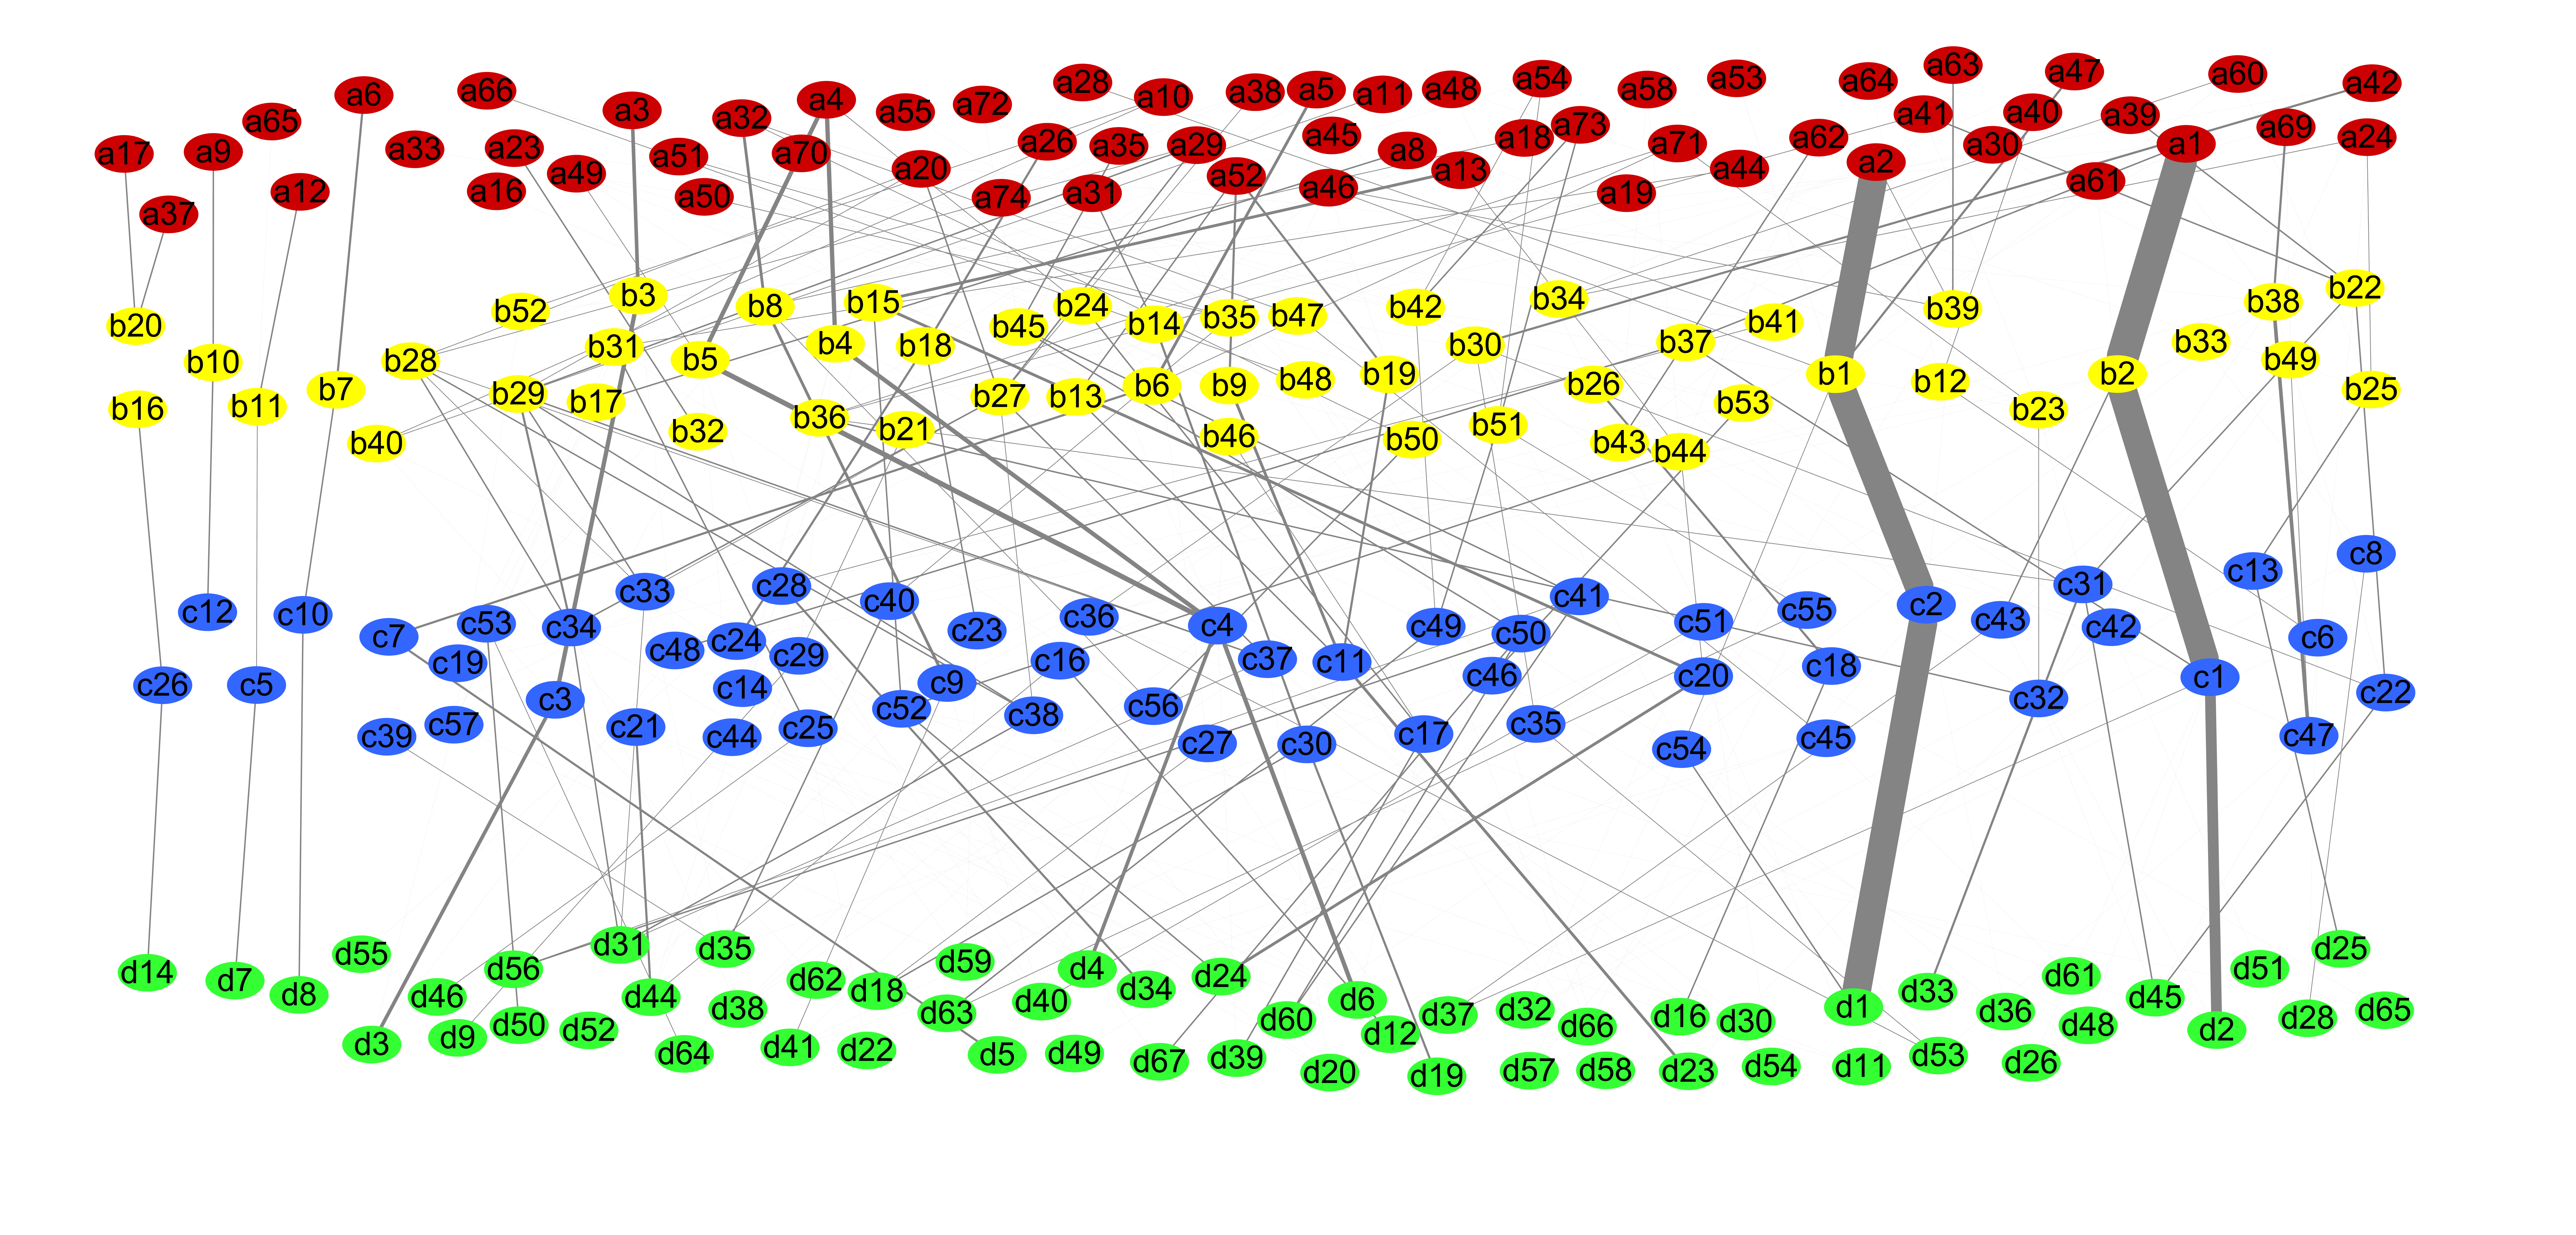
\includegraphics[width = .9\textwidth,height=6.5cm]{FIG/fig3.png}
	\caption{Modules relation network between adjacent stages of CRC. Red, yellow, blue, and green circles represent modules belonging to DEG-stage1, DEG-stage2, DEG-stage3, and DEG-stage4, respectively.}
	\label{Fig3}
\end{figure*}

\section*{Acknowledgment}
This work was supported by the National Natural Science Foundation of China under [Grant No. 61602386, 61972320, 61702161 and 61772426]; 
the Natural Science Foundation of Shaanxi Province under [Grant No. 2017JQ6008]; 
the Fundamental Research Funds for the Central Universities under [Grant No. 3102019DX1003];  
and the Top International University Visiting Program for Outstanding Young scholars of Northwestern Polytechnical University.


\bibliographystyle{IEEEtran}
\bibliography{IEEEabrv,temp-paper}
%\vspace{12pt}
\end{document}
